\RequirePackage{shellesc}
\immediate\write18{tex penrose_code.dtx}
\immediate\write18{cd ../spath3-git; tex spath3_code.dtx}
\documentclass{article}

\usepackage[svgnames]{xcolor}
\usepackage{tikz}
\usetikzlibrary{penrose,spath3}

\tikzset{
  every Penrose pic/.style={draw,ultra thick},
  every circle arc/.style={draw,thin},
  every long arc/.style={draw,thin},
}

\makeatletter
\tikzset{
  tint fill colour/.code={%
    \edef\@temp{%
      \def\noexpand\tikz@fillcolor{\tikz@fillcolor!#1}%
      \noexpand\tikz@addoption{\noexpand\pgfsetfillcolor{\tikz@fillcolor!#1}}%
    }%
    \@temp
  }
}
\makeatother

\colorlet{thinRhombus}{DarkOrchid}
\colorlet{thickRhombus}{DarkSlateGray}
\colorlet{circleArc}{RosyBrown}
\colorlet{longArc}{LawnGreen}

\colorlet{kite}{HotPink}
\colorlet{dart}{Fuchsia}

\colorlet{goldenTriangle}{Gold}
\colorlet{reverseGoldenTriangle}{Magenta}
\colorlet{goldenGnomon}{Cyan}
\colorlet{reverseGoldenGnomon}{LimeGreen}


\begin{document}

\begin{tikzpicture}
\path[save Penrose path=a] (0,0) -- (.3,-.1) to[out=30,in=200] (1,0);
\path[save Penrose path=b] (0,0) -- (.3,-.1) to[out=30,in=180] (1,0);
\path[save Penrose path=c] (0,0) -- (.3,-.1) to[out=30,in=160] (1,0);
\path[save Penrose path=d] (0,0) -- (.3,-.1) to[out=30,in=140] (1,0);
\path[save Penrose path=e] (0,0) -- (.3,-.1) to[out=30,in=120] (1,0);
\BakePenroseTile{kite}
\BakePenroseTile{dart}
\BakePenroseTile{thin rhombus}
\BakePenroseTile{thick rhombus}
\BakePenroseTile{pentagon 5}
\BakePenroseTile{pentagon 3}
\BakePenroseTile{pentagon 2}
\BakePenroseTile{pentagram}
\BakePenroseTile{boat}
\BakePenroseTile{diamond}
\BakePenroseTile{golden triangle}
\BakePenroseTile{reverse golden triangle}
\BakePenroseTile{golden gnomon}
\BakePenroseTile{reverse golden gnomon}
\end{tikzpicture}

\begin{tikzpicture}
\draw[help lines] (0,1) grid (2,5);
\foreach[count=\k] \pth in {a,b,c,d,e}
{
  \node[left] at (0, \k) {\pth};
  \draw[spath/set name=Penrose, spath/transform={\pth}{yshift=\k cm, scale=1cm/1pt}, spath/restore=\pth];
}
\foreach[count=\k] \pth in {A,B,C,D,E}
{
  \draw[spath/set name=Penrose, spath/transform={\pth}{yshift=\k cm, xshift= 1cm, scale=1cm/1pt}, spath/restore=\pth];
}
\end{tikzpicture}

\section{Kites and Darts}

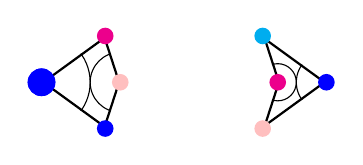
\begin{tikzpicture}
\pic[kite,name=tile];
\fill[blue] (0,0) circle[radius=5pt];
\foreach \edg/\col/\opp in {a/cyan/A, c/magenta/C, A/blue/a, C/pink/c}
{
  \fill[\col] (0,0) (tile-edge \edg\space start) circle[radius=3pt];
}
\pic[every Penrose pic, name=tile] at (3,0) {dart};
\fill[blue] (0,0) circle[radius=5pt];
\foreach \edg/\col/\opp in {a/cyan/A, c/magenta/C, A/blue/a, C/pink/c}
{
  \fill[\col] (0,0) (tile-edge \edg\space start) circle[radius=3pt];
}
\end{tikzpicture}

\subsection{Alignments}

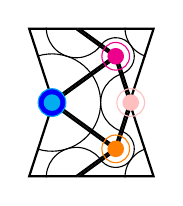
\begin{tikzpicture}
\pic[kite,name=tile];
\pic[dart,align with=tile along c, name=ctile];
\pic[kite,align with=tile along a, name=atile];
\pic[kite,align with=tile along A, name=Atile];
\pic[dart,align with=tile along C, name=Ctile];
\fill[blue] (0,0) circle[radius=5pt];
\foreach \edg/\col/\opp in {a/cyan/A, c/magenta/C, A/orange/a, C/pink/c}
{
  \fill[\col] (0,0) (tile-edge \edg\space start) circle[radius=3pt];
  \draw[\col] (0,0) (\edg tile-edge \opp\space end) circle[radius=5pt];
}
\end{tikzpicture}

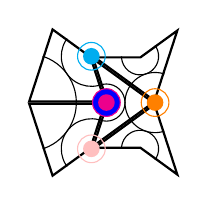
\begin{tikzpicture}
\pic[dart,name=tile];
\pic[kite,align with=tile along c, name=ctile];
\pic[dart,align with=tile along a, name=atile];
\pic[dart,align with=tile along A, name=Atile];
\pic[kite,align with=tile along C, name=Ctile];
\fill[blue] (0,0) circle[radius=5pt];
\foreach \edg/\col/\opp in {a/cyan/A, c/magenta/C, A/orange/a, C/pink/c}
{
  \fill[\col] (0,0) (tile-edge \edg\space start) circle[radius=3pt];
  \draw[\col] (0,0) (\edg tile-edge \opp\space end) circle[radius=5pt];
}
\end{tikzpicture}

\subsection{Decomposition}

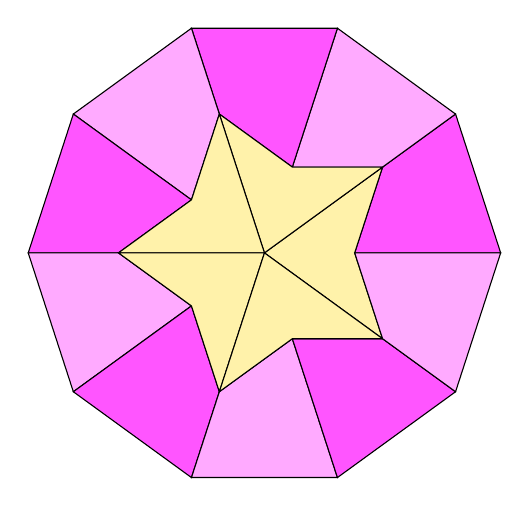
\begin{tikzpicture}[
  every Penrose tile/.style={draw},
  every golden triangle/.style={fill=goldenTriangle},
  every reverse golden triangle/.style={fill=reverseGoldenTriangle},
  every golden gnomon/.style={fill=goldenGnomon},
  every reverse golden gnomon/.style={fill=reverseGoldenGnomon},
  every kite/.style={fill=reverseGoldenTriangle},
  every dart/.style={fill=goldenTriangle},
  Penrose tile/.code 2 args={
    \pgfmathsetmacro\tint{100*(1 - #1/(1.5*#2))}
    \pgfkeysalso{tint fill colour=\tint}
%    \message{#1 and #2,}
  }
]
\foreach[evaluate=\k as \mk using {\k+Mod(\k,2)},evaluate=\k as \ax using {Mod(\k,2) == 0 ? "T" : "t"}] \k in {0,...,9} {
  \begin{scope}[rotate=\mk*36]
  \PenroseDecomposition[Penrose step=3cm]{kite}{1}{\ax}
  \end{scope}
}
\end{tikzpicture}


\section{Rhombii}

\subsection{Alignments}

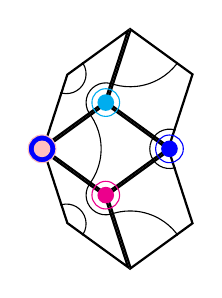
\begin{tikzpicture}
\pic[thick rhombus,name=tile];
\pic[thin rhombus,align with=tile along b, name=btile];
\pic[thick rhombus,align with=tile along a, name=atile];
\pic[thick rhombus,align with=tile along A, name=Atile];
\pic[thin rhombus,align with=tile along B, name=Btile];
\fill[blue] (0,0) circle[radius=5pt];
\foreach \edg/\col/\opp in {a/cyan/A, b/magenta/B, A/blue/a, B/pink/b}
{
  \fill[\col] (0,0) (tile-edge \edg\space start) circle[radius=3pt];
  \draw[\col] (0,0) (\edg tile-edge \opp\space end) circle[radius=5pt];
}
\end{tikzpicture}

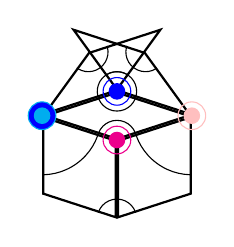
\begin{tikzpicture}
\pic[thin rhombus,name=tile];
\pic[thick rhombus,align with=tile along b, name=btile];
\pic[thin rhombus,align with=tile along a, name=atile];
\pic[thin rhombus,align with=tile along A, name=Atile];
\pic[thick rhombus,align with=tile along B, name=Btile];
\fill[blue] (0,0) circle[radius=5pt];
\foreach \edg/\col/\opp in {a/cyan/A, b/magenta/B, A/blue/a, B/pink/b}
{
  \fill[\col] (0,0) (tile-edge \edg\space start) circle[radius=3pt];
  \draw[\col] (0,0) (\edg tile-edge \opp\space end) circle[radius=5pt];
}
\end{tikzpicture}

\subsection{Decomposition}

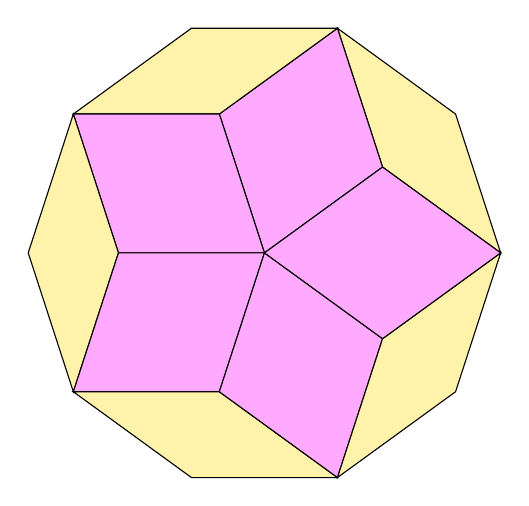
\begin{tikzpicture}[
  every Penrose tile/.style={draw},
  every golden triangle/.style={fill=goldenTriangle},
  every reverse golden triangle/.style={fill=reverseGoldenTriangle},
  every golden gnomon/.style={fill=goldenGnomon},
  every reverse golden gnomon/.style={fill=reverseGoldenGnomon},
  every thick rhombus/.style={fill=reverseGoldenTriangle},
  every thin rhombus/.style={fill=goldenTriangle},
  Penrose tile/.code 2 args={
    \pgfmathsetmacro\tint{100*(1 - #1/(1.5*#2))}
    \pgfkeysalso{tint fill colour=\tint}
%    \message{#1 and #2,}
  }
]
\foreach[evaluate=\k as \mk using {\k+Mod(\k,2)},evaluate=\k as \ax using {Mod(\k,2) == 0 ? "T" : "t"}] \k in {0,...,9} {
  \begin{scope}[rotate=\mk*36]
  \PenroseDecomposition[Penrose step=3cm]{rhombus}{1}{\ax}
  \end{scope}
}
\end{tikzpicture}



\end{document}

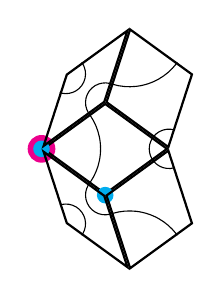
\begin{tikzpicture}
\fill[magenta] (0,0) circle[radius=5pt];
\pic[thick rhombus,name=tile];
\fill[cyan] (0,0) (tile-edge b start) circle[radius=3pt];
\fill[cyan] (0,0) (tile-edge b end) circle[radius=3pt];
\pic[thin rhombus,align with=tile along b];
\pic[thick rhombus,align with=tile along a];
\pic[thick rhombus,align with=tile along A];
\pic[thin rhombus,align with=tile along B];
\end{tikzpicture}

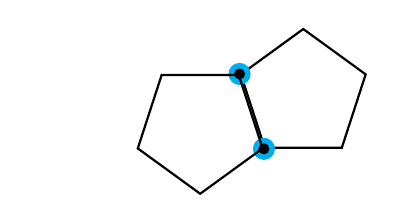
\begin{tikzpicture}
\pic[pentagon 5,name=ptile,at={(3,0)}];
\fill[cyan] (0,0) (ptile-edge a1 start) circle[radius=4pt];
\fill[cyan] (0,0) (ptile-edge a1 end) circle[radius=4pt];
\pic[pentagon 3,align with=ptile along a1,name=qtile];
\fill (0,0) (qtile-edge A start) circle[radius=2pt];
\fill (0,0) (qtile-edge A end) circle[radius=2pt];
\end{tikzpicture}

\end{document}
